\documentclass[11pt,a4paper]{article}

\usepackage[utf8]{inputenc}
\usepackage[T1]{fontenc}
\usepackage{lmodern}
\usepackage[margin=2.5cm]{geometry}
\usepackage{amsmath,amssymb}
\usepackage{booktabs}
\usepackage{multirow}
\usepackage{graphicx}
\usepackage{caption}
\usepackage[round]{natbib}
\usepackage[hidelinks]{hyperref}

\graphicspath{{../figures/}}

\title{Predicting Golden Cross Transitions in ETFs:\\What Survives a Careful Evaluation}
\author{Alexandre Galle\\Independent Researcher\\\texttt{alexandre.galle@student-cs.fr}}
\date{October 2026}

\begin{document}
\maketitle

\begin{abstract}
We study whether machine-learning classifiers can anticipate, up to 30 trading days ahead,
crossovers between the 50-day and 200-day simple moving averages (Golden and Death Crosses)
of exchange-traded funds. XGBoost and Random Forest classifiers are trained on SPY with
12 technical and moving-average features over 2000--2024 and applied without retraining to
DIA, QQQ, GLD and TLT. Under a first evaluation protocol, in which the decision threshold is
selected on the test set and confidence intervals assume independent observations, XGBoost
reaches a mean F1 of 0.738 on SPY, DIA and QQQ. We then correct three weaknesses of this protocol.
Selecting the threshold on a validation block inside the training period, with a 30-day embargo,
lowers the mean F1 to 0.595 for XGBoost and 0.633 for Random Forest. A moving-block bootstrap that
respects the 30-day autocorrelation of the labels makes the confidence intervals 2.6 to 3.7
times wider. Finally, a rule with no learned parameters, which linearly extrapolates the gap between
the two moving averages, obtains a mean F1 of 0.720 and exceeds both models on three of the five
assets. Each test set contains only 5 to 10 crossover events, and XGBoost results move by
up to 0.047 in mean F1 when prices are perturbed by one part in a million. We conclude that
crossover timing over a 30-day horizon is largely predictable from the mechanics of the moving
averages themselves, and that the apparent contribution of the classifiers is mostly an artefact
of the first protocol.
\end{abstract}

\section{Introduction}

Moving-average crossover rules are among the most widely used trend indicators. They are usually
studied as reactive signals: a position changes once the crossover has occurred
\citep{avramov2018}. The 50/200-day pair, known as the Golden Cross (upward) and Death Cross
(downward), is the most common long-horizon variant, and the ratio between these two averages
carries information about future returns \citep{bhootra2023}. A natural question is whether the
crossover itself can be anticipated.

This paper started as an attempt to answer that question with gradient boosting and random
forests. A first round of experiments suggested a positive answer, with F1 scores around 0.74.
Closer inspection showed that this figure depended on choices that a careful reviewer would
reject. The paper therefore reports the full path from the first estimate to a corrected one.

Our contributions are:
\begin{enumerate}
  \item a reproducible pipeline for predicting MA50/MA200 crossovers 30 days ahead, trained on
        SPY and transferred to four other ETFs;
  \item a decomposition of how the evaluation protocol inflates performance: threshold selection
        on the test set and observation-level bootstrap intervals;
  \item a parameter-free extrapolation baseline that matches the learned models, showing that the
        target is largely predictable by construction;
  \item an account of the statistical limits of the setting: few independent events per test set,
        threshold instability across time, and sensitivity to negligible numerical perturbations.
\end{enumerate}

Section~\ref{sec:related} reviews related work. Section~\ref{sec:data} describes the data and
target. Section~\ref{sec:method} presents the features, models and evaluation protocols.
Section~\ref{sec:results} reports results and Section~\ref{sec:discussion} discusses limitations.

\section{Related Work}\label{sec:related}

The distance or ratio between short- and long-term moving averages captures changes in price
regimes and predicts future returns \citep{avramov2018,bhootra2023}. Gradient boosting
\citep{chen2016} and other tree ensembles perform competitively in stock direction prediction
\citep{ampomah2020}. Transitions between bull and bear phases tend to coincide with elevated
volatility and trading activity \citep{catao2010}, which motivates part of our feature set.

On the evaluation side, labels built from future windows overlap in time, so information leaks
across a train/test boundary unless observations near it are purged or embargoed
\citep{lopezdeprado2018}. For dependent observations, resampling individual points underestimates
variance; block bootstrap methods resample contiguous segments instead \citep{kunsch1989}. Our
corrected protocol applies both ideas.

\section{Data and Target}\label{sec:data}

\subsection{Data}

We use daily Open-High-Low-Close prices and volumes from Yahoo Finance (\texttt{yfinance},
dividend-adjusted) for SPY, DIA, QQQ, GLD and TLT, together with the CBOE Volatility Index (VIX),
from 3 January 2000 to 30 December 2024. GLD and TLT start later (18 November 2004 and
30 July 2002). The models are trained on SPY only. Table~\ref{tab:data} summarizes the samples
after removing the first rows, for which the 200-day average and other rolling windows are
undefined.

Adjusted prices returned by \texttt{yfinance} differ slightly between successive downloads:
on SPY, 5{,}378 of 6{,}288 closing prices differed between two calls, by at most \$0.0002. All
results below use a single cached snapshot of the data so that runs are reproducible.
Section~\ref{sec:sensitivity} measures how much these differences matter.

\begin{table}[h]
\centering
\begin{tabular}{lrrlrr}
\toprule
Asset & Train rows & Test rows & Test period & Positive rate (train / test) & Crossovers in test \\
\midrule
SPY & 4{,}563 & 1{,}521 & 2018-12-13 -- 2024-12-30 & 11.6\% / 9.9\% & 5 \\
DIA & 4{,}563 & 1{,}521 & 2018-12-13 -- 2024-12-30 & 15.1\% / 10.3\% & 6 \\
QQQ & 4{,}563 & 1{,}521 & 2018-12-13 -- 2024-12-30 & 14.4\% / 8.7\% & 5 \\
GLD & 3{,}643 & 1{,}215 & 2020-03-04 -- 2024-12-30 & 13.1\% / 22.5\% & 10 \\
TLT & 4{,}080 & 1{,}360 & 2019-08-06 -- 2024-12-30 & 20.3\% / 19.4\% & 9 \\
\bottomrule
\end{tabular}
\caption{Samples after a chronological 75/25 split per asset. Positive rate is the share of days
labeled 1. Crossovers are counted as events, not rows.}
\label{tab:data}
\end{table}

\subsection{A first target based on future returns}

We first labeled day $t$ as bullish when the return over the next $h$ days exceeded a threshold $r$:
\begin{equation}
  y_t = \mathbb{1}\left[\frac{P_{t+h}-P_t}{P_t} > r\right],
\end{equation}
over the grid $h\in\{15,30,60,90\}$ days and $r\in\{3\%,5\%,7\%,10\%\}$. The configuration
$h=60$, $r=5\%$ labels 36.7\% of days as bullish but switches 440 times between 2000 and 2024,
far more than the number of genuine market regimes. It also misses sustained trends: only 33.8\%
of days in the 2013--2017 bull market are labeled bullish (Figure~\ref{fig:target_return}).
We therefore abandoned this target.

\subsection{Moving-average regime and classification target}

The regime indicator is
\begin{equation}
  s_t = \mathbb{1}\left[\mathrm{MA}_{50}(t) > \mathrm{MA}_{200}(t)\right],
\end{equation}
where $\mathrm{MA}_k(t)$ is the $k$-day simple moving average of the closing price. On SPY it
changes 24 times over the period where both averages are defined, labels 71.9\% of days as
bullish, and covers 89.5\% of days in 2013--2017 (Figure~\ref{fig:target_gc}).

The classification target flags the 30 days that precede a regime change:
\begin{equation}
  y_t = \mathbb{1}\left[\exists\, i\in\{1,\dots,30\} : s_{t+i} \neq s_t\right].
  \label{eq:target}
\end{equation}
Positive days form contiguous blocks of 30, one block per crossover (two crossovers less than
30 days apart produce a merged block). Over the whole SPY sample, 11.1\% of days are positive.
The last 30 days of the sample cannot be labeled positive, since crossovers after
30 December 2024 are not observed.

\subsection{Robustness of the regime label}

We added Gaussian noise $\mathcal{N}(0,(\sigma\cdot\mathrm{sd}(P))^2)$ to the SPY price series,
where $\mathrm{sd}(P)$ is the standard deviation of the closing price over the sample, recomputed
$s_t$, and repeated this 50 times for each of 50 values of $\sigma\in[0.01,0.5]$. The absolute
change in the share of bullish days is at most 7.0\%, while the share of individual labels that
change rises from 0.5\% to 21.1\% (Figure~\ref{fig:noise}). The global regime structure is stable;
labels close to a crossover are sensitive to noise, as expected.

\section{Methodology}\label{sec:method}

\subsection{Features}

We use 12 features computed from past data only (Table~\ref{tab:features}). Raw price levels are
excluded because they are period-specific. Two features, ATR and MA velocity, are expressed in
price units, which matters when a model trained on SPY is applied to assets with different
price levels.

The moving-average features are
\begin{align}
  g_t &= \frac{\mathrm{MA}_{50}(t)-\mathrm{MA}_{200}(t)}{\mathrm{MA}_{200}(t)}, \\
  \text{MA\_velocity}_t &= \left[\mathrm{MA}_{50}(t)-\mathrm{MA}_{50}(t-5)\right]
                          -\left[\mathrm{MA}_{200}(t)-\mathrm{MA}_{200}(t-5)\right], \\
  \text{MA50\_slope}_t &= \frac{\mathrm{MA}_{50}(t)-\mathrm{MA}_{50}(t-10)}{\mathrm{MA}_{50}(t)}, \\
  \text{Distance\_normalized}_t &= \frac{g_t}{\frac{1}{50}\sum_{i=0}^{49}\sigma_{t-i}}, \\
  \text{MA\_cross\_momentum}_t &= \frac{\Delta_5\mathrm{MA}_{50}(t)-\Delta_{10}\mathrm{MA}_{50}(t)}{|g_t|},
\end{align}
where $\Delta_k\mathrm{MA}_{50}(t)=\mathrm{MA}_{50}(t)-\mathrm{MA}_{50}(t-k)$ and $\sigma_t$ is the
20-day realized volatility. The sign of $g_t$ equals the current regime $s_t$; this is not a leak of
the target, which concerns future changes of $s_t$, but it means the models know the current regime.

\begin{table}[h]
\centering
\begin{tabular}{ll}
\toprule
Feature & Definition \\
\midrule
Return & 1-day return \\
Volatility & standard deviation of daily returns over 20 days \\
Cumulated\_Return\_5d & compounded return over 5 days \\
RSI14 & relative strength index, 14 days, simple averages \\
Volume\_ROC & 14-day percentage change in volume \\
ATR & average true range, 14-day simple average \\
VIX\_spike & $\mathrm{VIX}_t$ divided by its 60-day moving average (including $t$) \\
Distance\_GC & $g_t$ \\
MA\_velocity, MA50\_slope, & \multirow{2}{*}{see equations above} \\
Distance\_normalized, MA\_cross\_momentum & \\
\bottomrule
\end{tabular}
\caption{Feature set.}
\label{tab:features}
\end{table}

\subsection{Models and hyperparameters}

We train an XGBoost classifier \citep{chen2016} with \texttt{scale\_pos\_weight} equal to the
ratio of negative to positive training days, and a Random Forest with balanced class weights.
Hyperparameters were selected by randomized search (100 configurations, \texttt{TimeSeriesSplit}
with 5 folds, F1 on the positive class) on the SPY training set only. For XGBoost, early stopping
with a patience of 30 rounds on the last validation fold reduced the number of trees from 327 to
138. Because this validation fold is also scored by the search, the selected XGBoost
configuration is slightly optimistic. Tables~\ref{tab:hp_xgb} and~\ref{tab:hp_rf} report the
values used in all experiments; the search is in notebook \texttt{02} of the repository.

\begin{table}[h]
\centering
\begin{minipage}{0.45\textwidth}
\centering
\begin{tabular}{lr}
\toprule
Hyperparameter & Value \\
\midrule
n\_estimators & 138 \\
max\_depth & 5 \\
learning\_rate & 0.043 \\
subsample & 0.727 \\
colsample\_bytree & 0.698 \\
gamma & 0.054 \\
min\_child\_weight & 1 \\
\bottomrule
\end{tabular}
\caption{XGBoost (CV F1 0.659).}
\label{tab:hp_xgb}
\end{minipage}
\hfill
\begin{minipage}{0.45\textwidth}
\centering
\begin{tabular}{lr}
\toprule
Hyperparameter & Value \\
\midrule
n\_estimators & 346 \\
max\_depth & 9 \\
min\_samples\_split & 17 \\
min\_samples\_leaf & 5 \\
max\_features & 0.546 \\
\bottomrule
\end{tabular}
\caption{Random Forest (CV F1 0.638).}
\label{tab:hp_rf}
\end{minipage}
\end{table}

\subsection{Evaluation protocols}

Each asset is split chronologically: the first 75\% of rows form the training set, the last 25\%
the test set. Models are trained on SPY and applied unchanged to the other assets, using the
threshold selected on SPY. We compare two protocols.

\paragraph{Naive protocol.} The model is trained on the full SPY training set. The decision
threshold is the value in $\{0.10, 0.15, \dots, 0.95\}$ that maximizes F1 on the SPY test set.
Confidence intervals come from a bootstrap that resamples individual days. This reproduces the
first version of this study.

\paragraph{Corrected protocol.} The last 20\% of the SPY training set (913 days, 30 April 2015 to
12 December 2018, containing 5 crossovers) is held out for validation. A model trained on the
earlier days, minus a 30-day embargo before the validation block, selects the threshold that
maximizes validation F1. The final model is then trained on the full training set minus its last
30 days, whose labels depend on test-period prices \citep{lopezdeprado2018}. Confidence intervals
come from a moving-block bootstrap with blocks of 30 days \citep{kunsch1989}. Both bootstraps use
$B=1000$ resamples and percentile intervals at 95\%.

\subsection{Baselines}

\paragraph{Extrapolation rule.} Let $\dot g_t = (g_t - g_{t-5})/5$. If the gap kept its recent
trend, it would reach zero after $\tau_t = -g_t/\dot g_t$ days. The rule predicts
\begin{equation}
  \hat y_t = \mathbb{1}\left[0 < \tau_t \le 30\right].
\end{equation}
The horizon equals the target horizon, and a search over $\{5,10,\dots,90\}$ on the SPY training
set also selects 30, so the rule has no learned parameter. Its rationale is mechanical:
$\mathrm{MA}_{200}(t+30)$ shares 170 of its 200 prices with information available at $t$.

\paragraph{Stratified random.} Predicting 1 at random with the training positive rate $p$ gives an
expected F1 of $2pq/(p+q)$, where $q$ is the test positive rate.

\subsection{Additional analyses}

\paragraph{Walk-forward.} On the full SPY series, we use an expanding training window starting
at 50\% of the sample and five test folds of 608 days. In each fold, the threshold is re-selected
on the last 20\% of the current training window with the same embargo. Folds with fewer than two
positive days are skipped.

\paragraph{Numerical sensitivity.} We multiply all SPY, DIA and QQQ prices by $(1+\varepsilon_t)$,
$\varepsilon_t\sim\mathcal{N}(0,10^{-12})$, i.e. relative perturbations of order $10^{-6}$, similar
to the differences between two \texttt{yfinance} downloads, and rerun the corrected protocol
20 times.

\section{Results}\label{sec:results}

\subsection{Naive protocol}

Under the naive protocol, the test-optimal thresholds are 0.90 for XGBoost and 0.65 for Random
Forest. Mean F1 over SPY, DIA and QQQ is 0.738 for XGBoost and 0.720 for Random Forest
(Table~\ref{tab:naive}). These figures are close to those of the first version of this study,
which used another download of the same data and found a test-optimal XGBoost threshold of 0.85.

\begin{table}[h]
\centering
\begin{tabular}{lcc}
\toprule
Asset & XGBoost ($\tau=0.90$) & Random Forest ($\tau=0.65$) \\
\midrule
SPY & 0.762 [0.698, 0.815] & 0.763 [0.709, 0.810] \\
DIA & 0.683 [0.618, 0.740] & 0.653 [0.592, 0.706] \\
QQQ & 0.769 [0.705, 0.824] & 0.745 [0.685, 0.798] \\
GLD & 0.661 [0.600, 0.713] & 0.737 [0.693, 0.776] \\
TLT & 0.618 [0.558, 0.676] & 0.643 [0.596, 0.683] \\
\midrule
Mean SPY/DIA/QQQ & 0.738 & 0.720 \\
\bottomrule
\end{tabular}
\caption{Naive protocol: F1 with observation-level bootstrap 95\% intervals. Thresholds are
selected on the SPY test set.}
\label{tab:naive}
\end{table}

\subsection{Corrected protocol}

On the validation block, the selected thresholds are 0.20 for XGBoost (validation F1 0.792) and
0.45 for Random Forest (0.760). Table~\ref{tab:main} reports test results. Mean F1 over SPY, DIA
and QQQ falls to 0.595 for XGBoost and 0.633 for Random Forest
(Figure~\ref{fig:protocol}). The drop comes from precision: with the lower thresholds, XGBoost
flags 291 SPY test days for 150 positive days, against 139 for the extrapolation rule.

\begin{table}[h]
\centering
\small
\begin{tabular}{lccccc}
\toprule
Asset & Model & Precision & Recall & F1 [95\% block CI] & Days flagged \\
\midrule
SPY & XGBoost & 0.457 & 0.887 & 0.603 [0.384, 0.771] & 291 \\
    & Random Forest & 0.535 & 0.820 & 0.647 [0.426, 0.794] & 230 \\
    & Extrapolation & 0.748 & 0.693 & 0.720 [0.489, 0.865] & 139 \\
    & Stratified & & & 0.106 & \\
\midrule
DIA & XGBoost & 0.415 & 0.834 & 0.554 [0.324, 0.692] & 316 \\
    & Random Forest & 0.533 & 0.828 & 0.648 [0.409, 0.782] & 244 \\
    & Extrapolation & 0.609 & 0.586 & 0.597 [0.382, 0.769] & 151 \\
    & Stratified & & & 0.109 & \\
\midrule
QQQ & XGBoost & 0.468 & 0.947 & 0.627 [0.393, 0.788] & 267 \\
    & Random Forest & 0.457 & 0.886 & 0.603 [0.341, 0.766] & 256 \\
    & Extrapolation & 0.853 & 0.833 & 0.843 [0.678, 0.931] & 129 \\
    & Stratified & & & 0.099 & \\
\midrule
GLD & XGBoost & 0.643 & 0.971 & 0.774 [0.643, 0.877] & 412 \\
    & Random Forest & 0.696 & 0.938 & 0.799 [0.679, 0.891] & 368 \\
    & Extrapolation & 0.786 & 0.740 & 0.762 [0.637, 0.860] & 257 \\
    & Stratified & & & 0.153 & \\
\midrule
TLT & XGBoost & 0.459 & 0.811 & 0.586 [0.413, 0.711] & 466 \\
    & Random Forest & 0.526 & 0.780 & 0.628 [0.448, 0.748] & 392 \\
    & Extrapolation & 0.783 & 0.723 & 0.752 [0.583, 0.853] & 244 \\
    & Stratified & & & 0.145 & \\
\midrule
\multicolumn{2}{l}{Mean SPY/DIA/QQQ} & & & XGB 0.595 / RF 0.633 / Extr. 0.720 & \\
\bottomrule
\end{tabular}
\caption{Corrected protocol: test results with 30-day moving-block bootstrap intervals.
Stratified is the expected F1 of random predictions.}
\label{tab:main}
\end{table}

\subsection{Comparison with the extrapolation rule}

The extrapolation rule obtains the highest F1 on SPY, QQQ and TLT. Random Forest is ahead on DIA,
and both models are ahead on GLD (Figure~\ref{fig:f1ci}). The block-bootstrap intervals of the
three methods overlap on every asset, so no per-asset ranking is statistically supported. All
methods are far above the stratified baseline.

Every method raises at least one alert within the 30 days before each of the 35 test crossovers.
The methods therefore differ in their false alarms, which determine precision.

Threshold-free ranking quality on SPY, measured by average precision, is 0.790 for XGBoost and
0.726 for Random Forest against a prevalence of 0.099 (Figure~\ref{fig:pr}). The probability
scores carry information; the difficulty lies in choosing a threshold that transfers from the
validation period to the test period.

\subsection{Uncertainty}

Block intervals are 2.6 to 3.7 times wider than observation-level intervals (3.3 on average
over the 15 asset-method pairs). For XGBoost on SPY, the observation-level interval is
$[0.547, 0.654]$ and the block interval $[0.384, 0.771]$. Positive days come in blocks of 30, so resampling
individual days treats one crossover as 30 independent observations. With 5 to 10 crossovers per
test set, one missed or spurious event changes F1 substantially.

\subsection{Walk-forward validation}

Table~\ref{tab:wf} reports the walk-forward results on SPY. Fold 1 (November 2012 to April 2015)
contains no positive day and is skipped. Pooled F1 over the four remaining folds is 0.651 for
XGBoost and 0.638 for Random Forest (Figure~\ref{fig:wf}). Fold F1 ranges from 0.387 to 0.792 and
the selected threshold from 0.10 to 0.80. Fold 5 contains a single crossover.

\begin{table}[h]
\centering
\begin{tabular}{lrrrcc}
\toprule
Fold & Train size & Positive days & Crossovers & XGBoost $\tau$ / F1 & Random Forest $\tau$ / F1 \\
\midrule
2 (2015-04 -- 2017-09) & 3{,}650 & 115 & 4 & 0.10 / 0.792 & 0.10 / 0.691 \\
3 (2017-09 -- 2020-02) & 4{,}258 & 68 & 2 & 0.15 / 0.562 & 0.40 / 0.642 \\
4 (2020-02 -- 2022-07) & 4{,}866 & 82 & 3 & 0.80 / 0.790 & 0.75 / 0.725 \\
5 (2022-07 -- 2024-12) & 5{,}474 & 30 & 1 & 0.40 / 0.387 & 0.45 / 0.420 \\
\midrule
Pooled & & & & 0.651 & 0.638 \\
\bottomrule
\end{tabular}
\caption{Walk-forward validation on SPY, expanding window, threshold re-selected in each fold.}
\label{tab:wf}
\end{table}

\subsection{Numerical sensitivity}\label{sec:sensitivity}

Over 20 runs with relative price perturbations of order $10^{-6}$, mean F1 over SPY, DIA and QQQ
is $0.609\pm0.012$ for XGBoost (range 0.596--0.643), $0.634\pm0.001$ for Random Forest and
0.720 for the extrapolation rule, which does not change. The selected XGBoost threshold varies
between 0.20 and 0.35. The likely source is \texttt{MA\_cross\_momentum}, which divides by
$|g_t|$ and amplifies small differences near a crossover.

\section{Discussion and Limitations}\label{sec:discussion}

\paragraph{What the results support.} Crossovers of the 50- and 200-day averages can be flagged
30 days in advance far better than chance. Most of this predictability follows from the
construction of the averages: a linear extrapolation of their gap reaches an F1 of 0.720 on SPY,
DIA and QQQ, and neither classifier exceeds it once the threshold is selected without access to
the test set.

\paragraph{Protocol effects.} Selecting the threshold on the test set raised mean F1 by 0.143 for
XGBoost and 0.087 for Random Forest. Observation-level bootstrap intervals were about three times
too narrow. Both effects are easy to miss when labels overlap in time.

\paragraph{Limitations.}
\begin{itemize}
  \item Each test set contains 5 to 10 crossovers, and the SPY, DIA and QQQ test sets cover the
        same dates on highly correlated assets. They are not independent confirmations.
  \item The selected threshold depends strongly on the period used for validation, as shown by
        the walk-forward folds.
  \item XGBoost results are sensitive to negligible numerical perturbations of the input data.
  \item Hyperparameters come from a search whose early stopping used a fold that the search also
        scored.
  \item ATR and MA velocity are not scale-free, which affects transfer to other assets.
  \item F1 on daily labels counts each crossover 30 times. An event-level metric that penalizes
        false alarms per unit of time would better reflect practical use.
  \item The study evaluates classification only. It does not evaluate a trading strategy,
        transaction costs or returns.
\end{itemize}

\paragraph{Future work.} A meaningful test of machine learning on this task should start from the
extrapolation rule and ask whether additional information, such as features unrelated to the
moving averages themselves, reduces false alarms. Longer horizons, where the mechanical overlap
between present and future averages is smaller, would also make the task less trivial.

\section{Conclusion}

A first evaluation suggested that XGBoost predicts Golden and Death Crosses 30 days ahead with an
F1 of about 0.74 and transfers across ETFs. With the threshold selected on validation data, an
embargo at the train/test boundary and block bootstrap intervals, F1 falls to about 0.6, and a
parameter-free extrapolation of the moving-average gap reaches 0.72. The modest result that
remains is that crossover timing at this horizon is largely mechanical, and that evaluation
choices can easily create the impression of a learned signal.

\paragraph{Reproducibility.} Code and all result tables are available at
\url{https://github.com/Bissapinho/Trend-classifier}. \texttt{scripts/run\_main.py} produces every number of
Section~\ref{sec:results} except Section~\ref{sec:sensitivity}, which comes from
\texttt{scripts/perturbation.py}; Section~\ref{sec:data} comes from
\texttt{scripts/target\_analysis.py}.

\begin{thebibliography}{9}

\bibitem[Ampomah et~al.(2020)]{ampomah2020}
Ampomah, E., Qin, Z., and Nyame, G. (2020).
\newblock Evaluation of tree-based ensemble machine learning models in predicting stock price
  direction of movement.
\newblock \emph{Information}, 11(6):332. doi:10.3390/info11060332.

\bibitem[Avramov et~al.(2018)]{avramov2018}
Avramov, D., Kaplanski, G., and Subrahmanyam, A. (2018).
\newblock Stock return predictability: New evidence from moving averages of prices and firm
  fundamentals.
\newblock \emph{SSRN Working Paper}.

\bibitem[Bhootra(2023)]{bhootra2023}
Bhootra, A. (2023).
\newblock Predicting returns using moving averages: the role of investor inattention.
\newblock \emph{Managerial Finance}, 50(6):1066--1088. doi:10.1108/MF-04-2023-0257.

\bibitem[Cat{\~a}o and Timmermann(2010)]{catao2010}
Cat{\~a}o, L. and Timmermann, A. (2010).
\newblock Volatility regimes and global equity returns.
\newblock In \emph{Volatility and Time Series Econometrics: Essays in Honor of Robert Engle}.
  Oxford University Press. doi:10.1093/acprof:oso/9780199549498.003.0013.

\bibitem[Chen and Guestrin(2016)]{chen2016}
Chen, T. and Guestrin, C. (2016).
\newblock XGBoost: A scalable tree boosting system.
\newblock In \emph{Proceedings of the 22nd ACM SIGKDD International Conference on Knowledge
  Discovery and Data Mining}, pages 785--794. doi:10.1145/2939672.2939785.

\bibitem[K{\"u}nsch(1989)]{kunsch1989}
K{\"u}nsch, H.~R. (1989).
\newblock The jackknife and the bootstrap for general stationary observations.
\newblock \emph{The Annals of Statistics}, 17(3):1217--1241.

\bibitem[L{\'o}pez de Prado(2018)]{lopezdeprado2018}
L{\'o}pez de Prado, M. (2018).
\newblock \emph{Advances in Financial Machine Learning}.
\newblock Wiley.

\end{thebibliography}

\clearpage
\appendix
\section{Figures}

\begin{figure}[h]
\centering
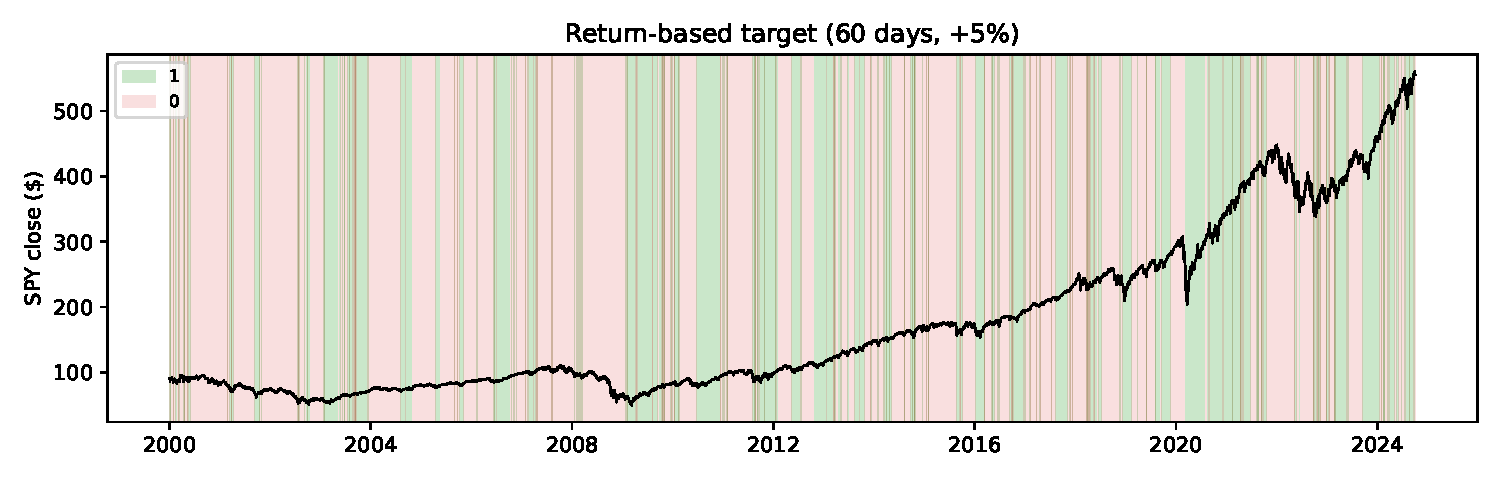
\includegraphics[width=\textwidth]{target_return.pdf}
\caption{Return-based target on SPY ($h=60$ days, $r=5\%$): 440 label switches over 2000--2024.}
\label{fig:target_return}
\end{figure}

\begin{figure}[h]
\centering
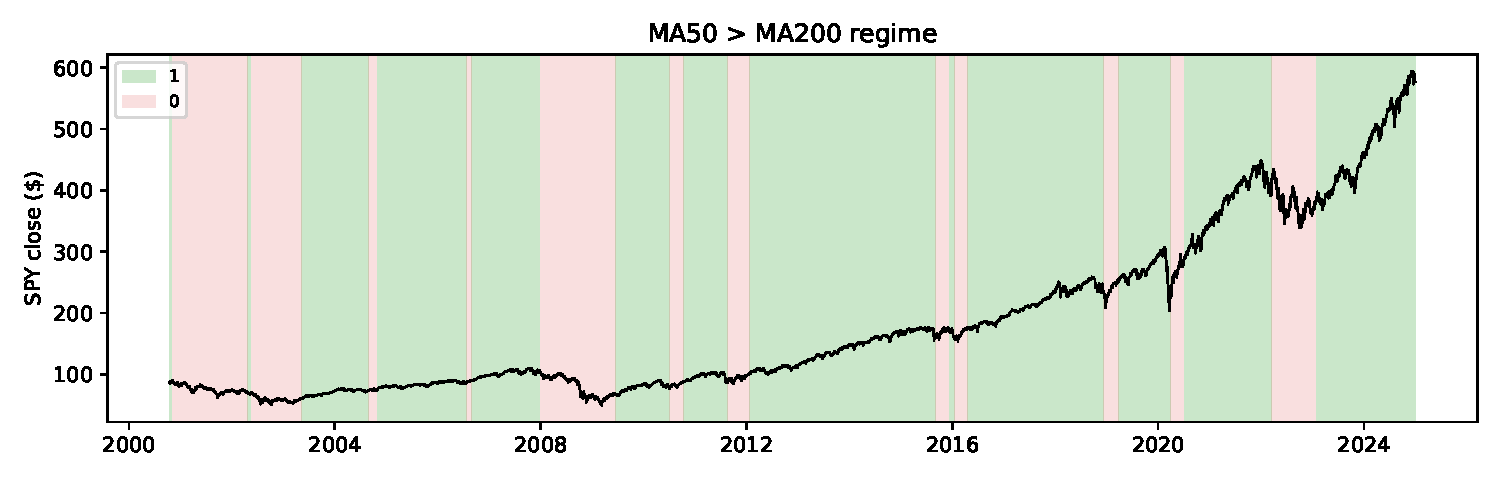
\includegraphics[width=\textwidth]{target_gc.pdf}
\caption{MA50/MA200 regime on SPY: 24 crossovers.}
\label{fig:target_gc}
\end{figure}

\begin{figure}[h]
\centering
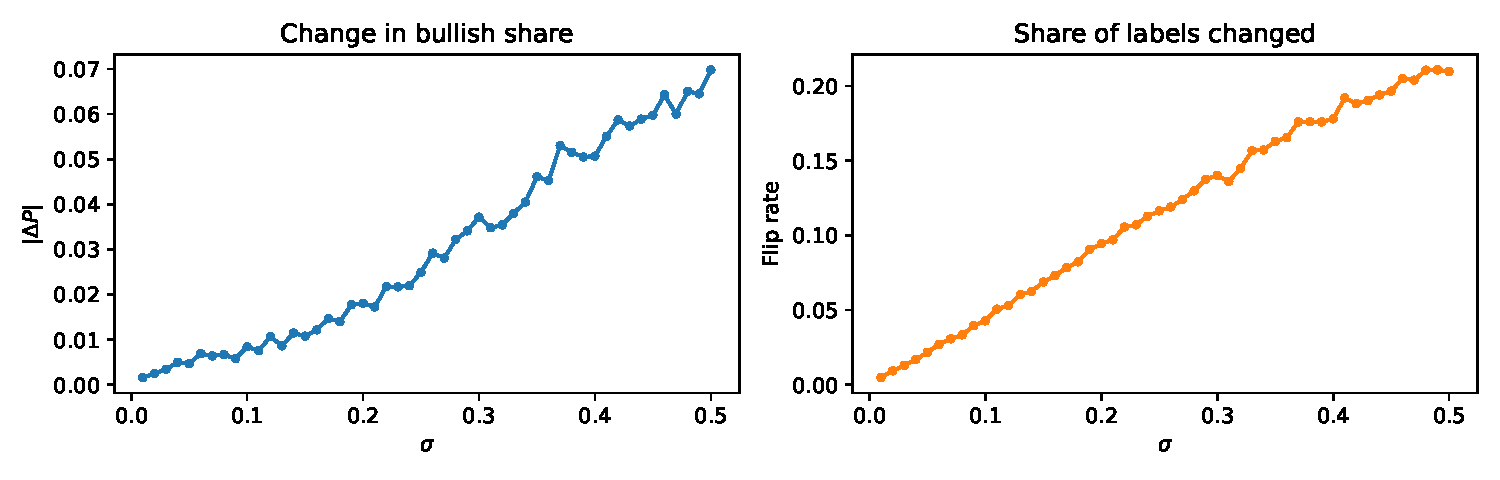
\includegraphics[width=\textwidth]{target_noise.pdf}
\caption{Noise robustness of the regime label: change in the share of bullish days (left) and
share of labels that change (right), averaged over 50 draws per $\sigma$.}
\label{fig:noise}
\end{figure}

\begin{figure}[h]
\centering
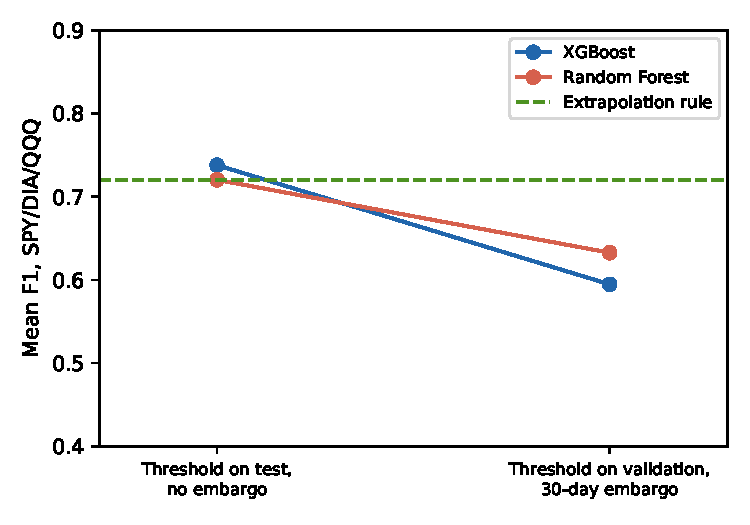
\includegraphics[width=0.6\textwidth]{protocol_effect.pdf}
\caption{Mean F1 over SPY, DIA and QQQ under the naive and corrected protocols, compared with the
extrapolation rule.}
\label{fig:protocol}
\end{figure}

\begin{figure}[h]
\centering
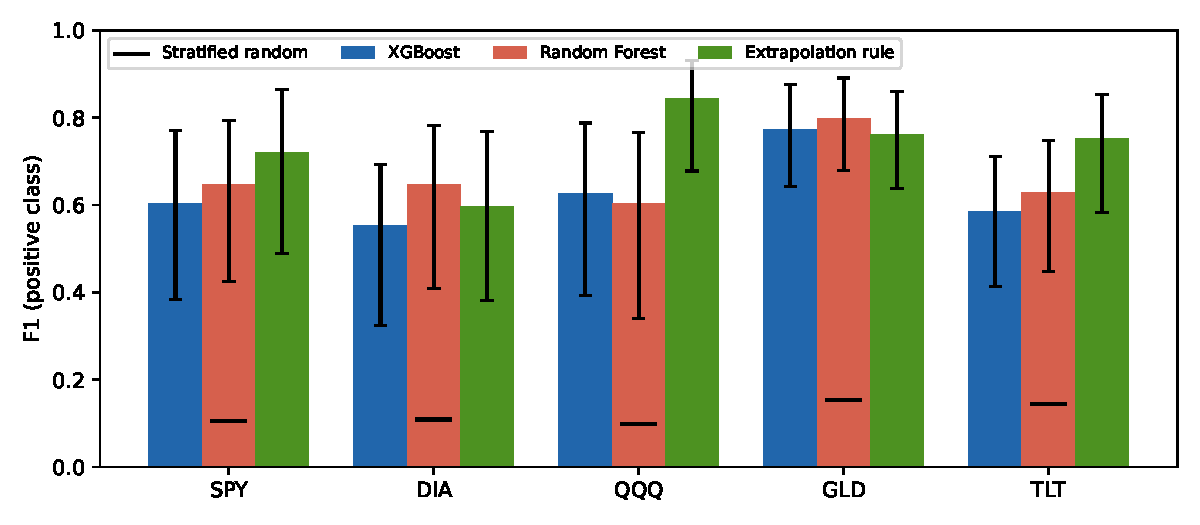
\includegraphics[width=\textwidth]{f1_block_ci.pdf}
\caption{Test F1 per asset under the corrected protocol, with 30-day block bootstrap 95\%
intervals. Black marks: expected F1 of stratified random predictions.}
\label{fig:f1ci}
\end{figure}

\begin{figure}[h]
\centering
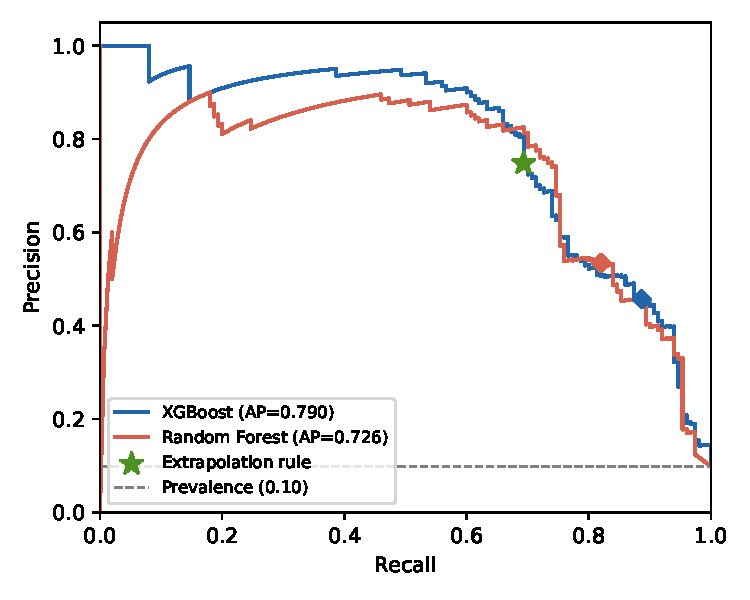
\includegraphics[width=0.6\textwidth]{pr_curve_spy.pdf}
\caption{Precision-recall curves on the SPY test set. Diamonds: operating points at the
validation-selected thresholds. Star: extrapolation rule. AP: average precision.}
\label{fig:pr}
\end{figure}

\begin{figure}[h]
\centering
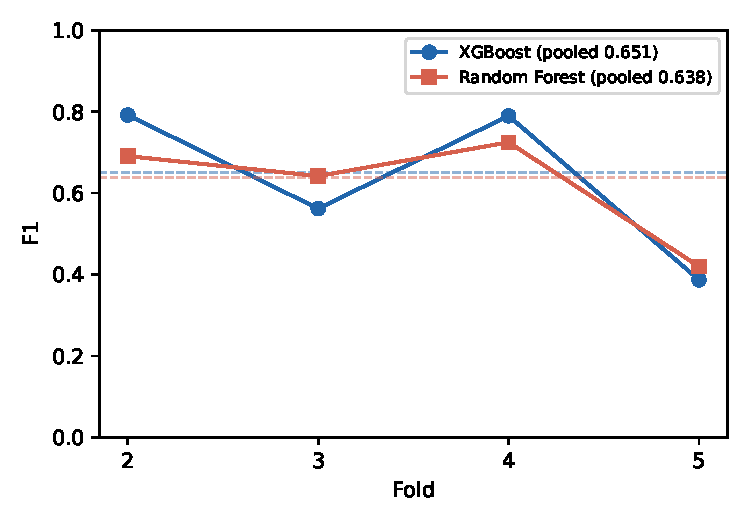
\includegraphics[width=0.6\textwidth]{walk_forward.pdf}
\caption{Walk-forward F1 per fold on SPY. Dashed lines: pooled F1.}
\label{fig:wf}
\end{figure}

\end{document}
